% Table 1 -  Maternal and Infant Characteristics by Racial Group of Infant
\begin{table}[ht]
\centering
\caption{Maternal and Infant Characteristics by Racial Group of Infant}
\label{tab:summary_table}
\begin{adjustbox}{max width=\textwidth}
\begin{tabular}{lll}
\toprule
& \textbf{Black Infants} & \textbf{White Infants} \\
\midrule
\multicolumn{3}{l}{\textbf{Count of Infants}} \\
\hspace{1em} N & 22,369 & 118,193 \\
\multicolumn{3}{l}{\textbf{Maternal Characteristics}} \\
\hspace{1em} Average Delivery Age & 27.39 & 28.27  \\
\hspace{1em}Age 15-19 & 0.00 (20) & 0.00 (48) \\
\hspace{1em}Age 20-24 & 0.08 (1733) & 0.05 (5623) \\
\hspace{1em}Age 25-29 & 0.28 (6210) & 0.22 (25821) \\
\hspace{1em}Age 30-34 & 0.30 (6632) & 0.32 (38090) \\
\hspace{1em}Age 35-39 & 0.22 (4814) & 0.28 (32763) \\
\hspace{1em}Age 40-44 & 0.10 (2344) & 0.11 (13216) \\
\hspace{1em}Age 45+ & 0.03 (616) & 0.02 (2632) \\
\hspace{1em}Any Prenatal Care & 0.68 (15321) & 0.62 (72783) \\
\hspace{1em}12+ Prenatal Visits & 0.24 (5465) & 0.19 (22988) \\
\hspace{1em}Mom Black & 0.80 (17937) & 0.01 (638) \\
\hspace{1em}Mom Other & 0.13 (2945) & 0.07 (7801) \\
\hspace{1em}Mom White & 0.07 (1487) & 0.93 (109754) \\
\hspace{1em}Medicaid & 0.59 (13108) & 0.26 (31285) \\
\hspace{1em}Other Insurance & 0.23 (5173) & 0.37 (43647) \\
\hspace{1em}Private Insurance & 0.18 (4088) & 0.37 (43261) \\
\hspace{1em}Maternal Chronic Pain Disorder & 0.06 (1305) & 0.04 (4968) \\
\hspace{1em}Maternal Gestational Diabetes & 0.07 (1673) & 0.08 (9304) \\
\hspace{1em}Maternal Gestational Hypertensive Disorder & 0.19 (4349) & 0.16 (19014) \\
\hspace{1em}Maternal Mental Health Disorder & 0.18 (4027) & 0.21 (24860) \\
\hspace{1em}Maternal Substance Use Disorder & 0.12 (2626) & 0.10 (11573) \\
\multicolumn{3}{l}{\textbf{Infant Characteristics}} \\
\hspace{1em}Average Crude Mortality Rate (2014-2018) per 10k & 2.71  & 2.03 \\
\hspace{1em}Average NAS Incidence per 100 Births & 0.01 & 0.01 \\
\hspace{1em}Average Number of Encounters Within 1 Month of Birth & 1.70  & 1.59  \\
\hspace{1em}Infant Tested & 0.16 (3690) & 0.07 (8655) \\
\hspace{1em}Infant Positive Test & 0.03 (745) & 0.01 (1707) \\
\hspace{1em}Low Birth Weight & 0.06 (1283) & 0.03 (3992) \\
\hspace{1em}Premature & 0.06 (1425) & 0.05 (5591) \\
\bottomrule
\end{tabular}
\end{adjustbox}
\end{table}



% Table 2 - Inverse Propensity Score Weighting Decomposition Results
\begin{table}[ht]
\centering
\caption{Observed and Reweighted Means, and Decomposition Results}
\label{tab:gap_testing_ipw}
\begin{tabular}{llrr}
  \toprule
  \multicolumn{4}{c}{\textbf{Panel A: Observed and Reweighted Means}} \\
  \cmidrule(lr){1-4}
  Group & White & Black \\ 
  \midrule
  Observed & 0.0732 & 0.1650 \\ 
  Reweighted & 0.1037 & 0.1295 \\ 
  \bottomrule
  \\
  \toprule
  \multicolumn{4}{c}{\textbf{Panel B: Decomposition Results (Reweighting Black Infants)}} \\
  \cmidrule(lr){1-4}
  Component & Gap & Standard Errors & Share of Raw Gap \\ 
  \midrule
  Raw Gap & 0.0917 &  & 1.0000 \\ 
  Reweighted Black - Observed White & 0.0563 & 0.0037 & 0.6138 \\ 
  Observed Black - Reweighted Black & 0.0354 & 0.0031 & 0.3862 \\ 
  \bottomrule
  \\
  \toprule
  \multicolumn{4}{c}{\textbf{Panel C: Decomposition Results (Reweighting White Infants)}} \\
  \cmidrule(lr){1-4}
  Component & Gap & Standard Errors & Share of Raw Gap \\ 
  \midrule
  Raw Gap & 0.0917 &  & 1.0000 \\ 
  Reweighted White - Observed White & 0.0305 & 0.0012 & 0.3320 \\ 
  Observed Black - Reweighted White & 0.0613 & 0.0029 & 0.6680 \\ 
  \bottomrule
\end{tabular}
\end{table}


% Figure 1 -- Testing rates and Postive testing rates over time by race.
\begin{landscape}
\begin{figure}[htbp]
    \centering
    \caption{Testing Rate and Positive Testing Rate by Racial Group of Infant by Year}
    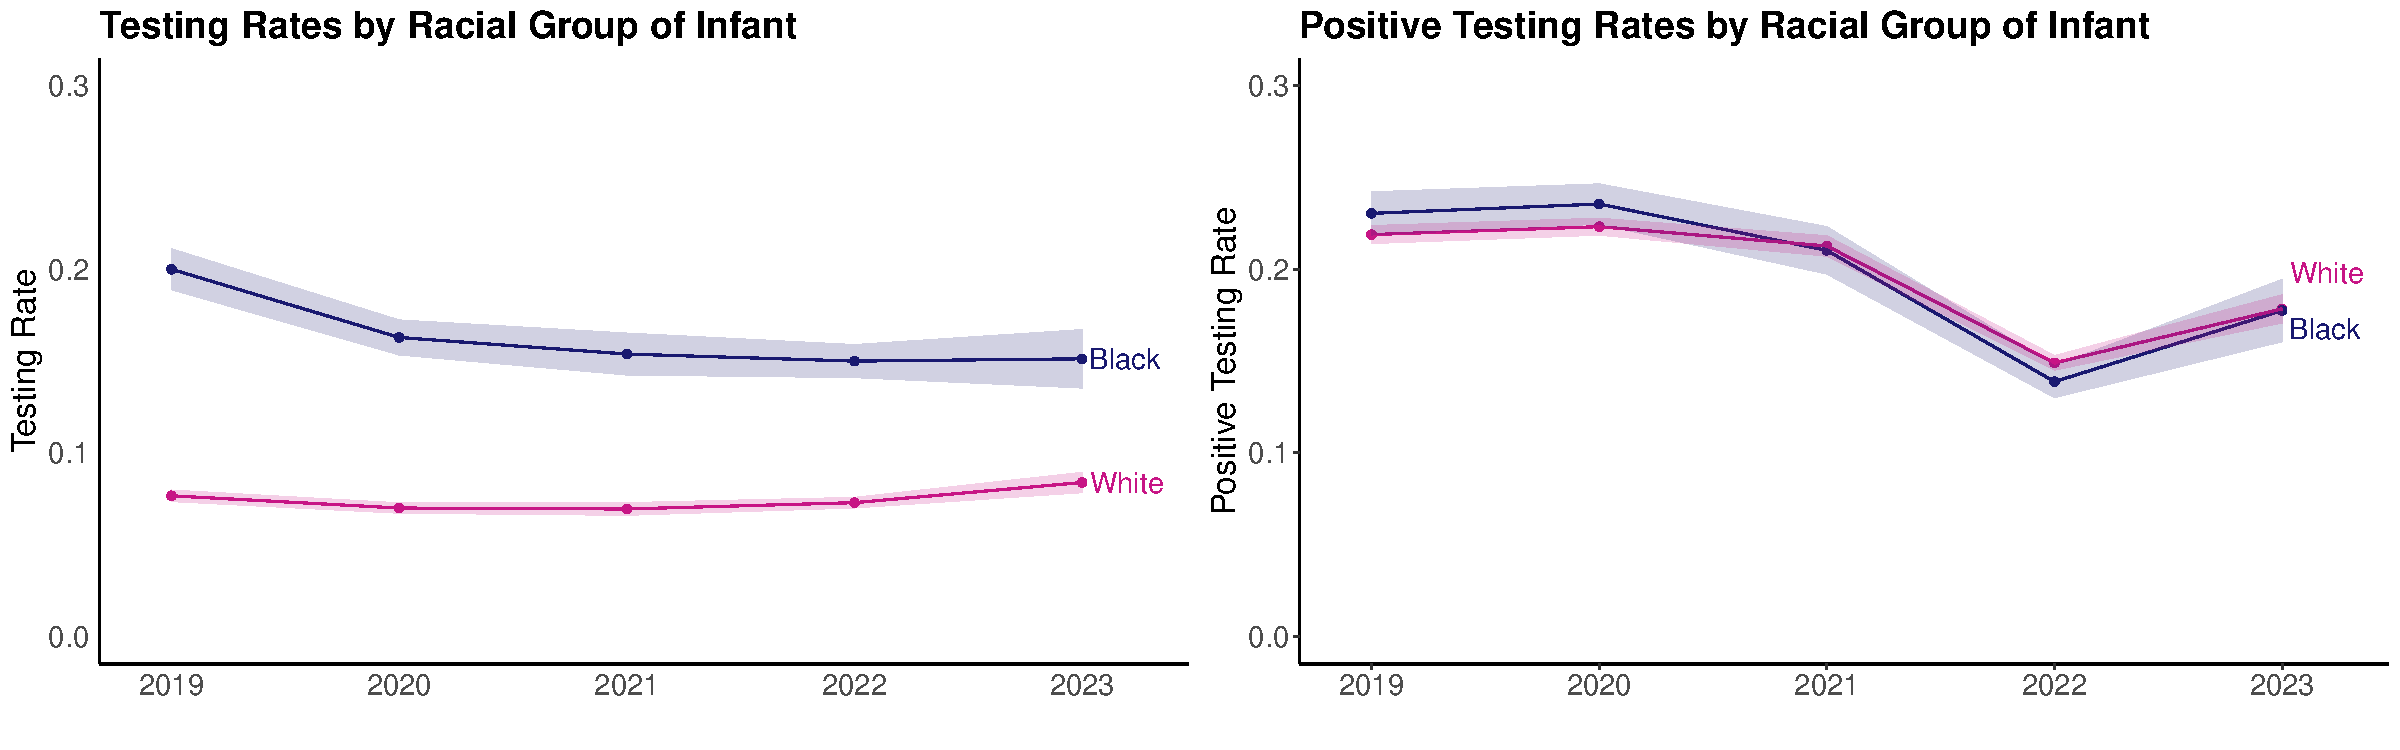
\includegraphics[width=1.3\textwidth]{../results/testing_race_year_race2.pdf}
    \label{fig:figure_1_testing_positive_by_year}
\small
\parbox{\linewidth}{
Note: The left panel shows the testing rate by year by racial group with the 95\% confidence interval. The right panel shows the positive testing rate by year by racial group with the 95\% confidence interval. The testing rate is calculated as the total number of infants tested divided by the total number of births in that year for each racial group. The positive testing rate is the number of infants with a positive test divided by the total number of infants tested in that year for each racial group.
}
\end{figure}
\end{landscape}

% Figure 2 -- Testing rates by maternal substance use history and race.
\begin{landscape}
    \begin{figure}[htbp]
    \centering
    \caption{Testing Rates by Racial Group of Infant and Maternal Substance Use History}
    
\includegraphics[width=1.3\textwidth]{../results/testing_rate_sud_history.pdf}
    \label{fig:figure_testing_sud}
    \centering
\small 
\parbox{\linewidth}{
Note: The left panel shows the testing rate by year by racial group of infant with mothers without a history of substance use disorder (those without any previous diagnosis code for SUD in the EMR data). The right panel shows the testing rate by year and racial group of infants with mothers with a history of SUD. The testing rate is calculated as the number of infants tested in the given year, racial group, and maternal substance use history divided by the total number of infants born that year in the given racial group and maternal substance use history category.
}
\end{figure}
\end{landscape}


% Figure 3 -- Positive test rates by maternal substance use history and race.
\begin{landscape}
    \begin{figure}[htbp]
    \centering
    \caption{Positive Testing Rates by Racial Group of Infant and Maternal Substance Use History}
    
\includegraphics[width=1.3\textwidth]{../results/positive_rate_sud_history.pdf}
    \label{fig:figure_positive_sud}
    \centering
\small 
\parbox{\linewidth}{
Note: The left panel shows the positive testing rate by year by racial group of infant for those with mothers without a history of substance use disorder (SUD). The right panel shows the positive testing rate by year by racial group of infant for those with mothers with a history of SUD. The positive testing rate is calculated as the number of infants with a positive test in the given year, racial group, and maternal substance use history category divided by the total number of infants tested for that group. 
}
\end{figure}
\end{landscape}

% Figure 4 -- County NAS and Testing Rates By Race
\begin{landscape}
    \begin{figure}[htbp]
    \centering
    \caption{Relationship between County NAS Incidence and County Average Testing Rate by Racial Group of Infant}
    
\includegraphics[width=1.3\textwidth]{../results/NAS_county_tested_all_weightbirths.pdf}
    \label{fig:figure_nas_test}
    \centering
\small 
\parbox{\linewidth}{
Note: The left panel shows the relationship between the testing rate among White infants in the infant's county of residence and the county-level neonatal abstinence syndrome incidence per 100 births (all racial groups). Each point in the figure shows the average testing rate among White infants and the NAS incidence per 100 births in that county, and the size of the dot is weighted by the number of births in that county. The fitted line is a weighted linear regression with weighting based on the number of infants born in the county. The coefficient from the regression is 0.049 which means that an increase in the county-level NAS incidence of 1 is correlated with an increase in the county-level testing rate of 4.9 percentage points among White infants. Similarly, the right panel shows the relationship between the county-level NAS incidence per 100 births with the county-level testing rate of Black infants. The coefficient from the weighted linear regression is 0.072, which means that a 1 unit increase in the NAS incidence per 100 births is associated with a 7.2 percentage point increase in the testing rate of Black infants. 
}
\end{figure}
\end{landscape}

% Figure 5 -- Average testing rates after reweighting
\begin{landscape}
\begin{figure}[htbp]    
\centering 
\caption{Average Testing Rate by Racial Group of Infant and Reweighted Black Average for Decomposition}

\includegraphics[width=1\textwidth]{../results/observed_reweighted_means_labeled.pdf}
\label{fig:testing_rates_reweighted}
\centering
\small
\parbox{\linewidth}{
Note:  This figure shows the average observed and reweighted testing rates by year to go along with the decomposition. The Black observed and White observed lines with the 95\% confidence intervals are the same as Figure 1. The Black reweighted line shows what the average testing rate for Black infants would be if they looked like White infants. The line is lower than the Black observed line but does not overlap with the White observed line. Across all years, the difference between the observed Black and reweighted Black testing rates accounts for 38.6\% of the difference in the observed Black and White testing rate. The difference between the reweighted Black and observed White average testing rates accounts for 61.4\% of the overall gap. 
}
\end{figure}
\end{landscape}